% CN: 分析实验附录；占位数据与实测结果必须显式区分。
% EN: Analysis-experiment appendix; placeholder data must be explicitly distinguished from measurements.
\section{\subsolver Component Ablations}
\label{app:pduot-component-ablation}
% CN: J=64 审计：本图全部 2598 次测量均保存重启计数，最大为 25，预算不会触发；保留原实验来源，不将其重标为已运行新保护版本。
% EN: J=64 audit: all 2598 measurements record restart counts, maximum 25, so the budget cannot trigger. Retain historical provenance rather than relabeling these runs as executions of the protected implementation. Evidence: experiments/primal_weight_budget_20261111/report/history_J64_audit.json.
We isolate the internal components of \subsolver on fixed restricted problems captured from TOME E11.5$\to$E12.5 runs with $m=n=65{,}536$ and $d=30$.
For each penalty pair, we increment the random seed from 42 and save every restricted solve across all hierarchy levels and refinement rounds until a completed parent run brings the corpus to at least 100 problems.
The four corpora contain 108, 106, 119, and 100 problems from 8, 7, 5, and 8 parent runs, respectively, in the panel order of Figure~\ref{fig:pduot-component-ablation-cdf}.
These include rectangular intermediate levels; problems from the same parent run are correlated.
Each variant is run once per snapshot with fixed support, costs, masses, output-translation policy, and an original restricted KKT tolerance of $10^{-6}$.

All six variants retain adaptive restart.
The weight ablation freezes the common initial primal weight $w_0$; the Halpern ablation removes anchor mixing while retaining reflection; and the reflection ablation retains Halpern anchoring.
The warm-start ablation zeros both the transport flow and dual potentials.
The preconditioning ablation replaces degree-based diagonal steps with scalar base steps under the same operator-norm safety bound and initial $w_0$.

\begin{figure}[htbp]
\centering
% CN: 图来自 paper_experiments_uot/pduot_ablation/results/pduot_cdf_n65536_seeds_20261110_gpu6/cdf_components_iterations.pdf；逐次结果与曲线数据分别见同目录 summary.json 和 cdf_data.json；采集来源为 results/corpus_n65536_seeds_20261110。
% EN: Figure source: paper_experiments_uot/pduot_ablation/results/pduot_cdf_n65536_seeds_20261110_gpu6/cdf_components_iterations.pdf; per-run results and curve data are summary.json and cdf_data.json in that directory; snapshots come from results/corpus_n65536_seeds_20261110.
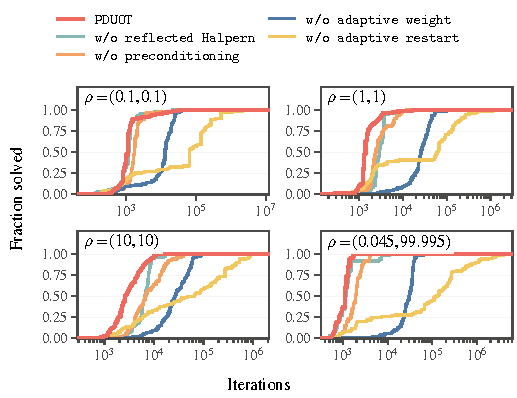
\includegraphics[width=0.96\linewidth]{figures/pduot_component_ablation_cdf_iterations.pdf}
\caption{\textbf{Internal \subsolver component ablations.}
Empirical CDFs of PDHG map evaluations to reach a restricted KKT residual of $10^{-6}$ on TOME snapshots ($d=30$, parent size $m=n=65{,}536$).
Panels separate the four penalty pairs; $N$ counts restricted problems, and curves farther left require fewer iterations.
Every variant retains adaptive restart, and each ablation removes only its named component.
The denominator includes all planned problems, including failures and timeouts; all 2,598 runs in this batch converged.}
\label{fig:pduot-component-ablation-cdf}
\end{figure}

Primal-weight updates, reflection, and diagonal preconditioning reduce total iteration counts in all four penalty settings.
Halpern anchoring helps at $(\rho_a,\rho_b)=(1,1)$ and $(10,10)$ and most strongly in the asymmetric setting, whereas removing it reduces total iterations at $(0.1,0.1)$.
Warm starts reduce total iterations in all four settings, although the corpus also includes coarsest problems whose initial flow and potentials are already zero.

\section{Primal-Weight Budget Intervention}
\label{app:pduot-weight-budget-experiment}

We compare complete TOME solves using the original controller and the budget in~\eqref{eq:pduot-weight-budget}.
This preliminary intervention uses $p=1.1$; the adopted default is $p=1.01$, $J=64$.
All runs use seed 42, $d=30$, \texttt{finest\_fp64} costs, the refinement safeguard, and KKT tolerance $10^{-6}$.
Every baseline and budgeted run converges.
The $J=1$ budget clips 19 updates and increases total iterations by up to $86\%$, mainly by restricting a coarse-level fallback recovery at $(0.1,0.1)$.
With $J=4$, two fallback updates are clipped without increasing iterations in any of these eight instances.
The $J=100$ control clips no updates and preserves every baseline iteration count.

% CN: 表中全部迭代数与裁剪次数来自 experiments/primal_weight_budget_20261111/report/small_J_iterations.json；原始记录为 results/J{1,4,100}_iterations_20261111/cases/*/{baseline,safe_clip}_trace_repeat0/metrics.json；完整性检查见 report/small_J_validation.json。
% EN: All iteration and clip counts come from experiments/primal_weight_budget_20261111/report/small_J_iterations.json; raw records are results/J{1,4,100}_iterations_20261111/cases/*/{baseline,safe_clip}_trace_repeat0/metrics.json; integrity checks are in report/small_J_validation.json.
% \xwz{RERUN REQUIRED: replace this preliminary whole-solve table (p=1.1) with iteration CDFs on the fixed restricted snapshots using the PDUOT component-ablation infrastructure, fixed p=1.01, default J=64, and smaller J values that actually trigger clipping. Include the original adaptive controller with the budget disabled as a separate baseline; frozen primal weight is not that baseline. Preserve all planned problems in CDF denominators, report clip counts and convergence failures, and retain the current data as historical provenance.}
\begin{table}[t]
\centering
\caption{\textbf{Preliminary weight-budget intervention.}
Total inner iterations across all hierarchy levels; parentheses count clipped weight updates.
Each configuration has one measurement at $p=1.1$.}
\label{tab:pduot-weight-budget}
\footnotesize
\setlength{\tabcolsep}{3pt}
\begin{tabular}{@{}lrrr@{}}
\toprule
$(\rho_a,\rho_b)$ & Original & $J=1$ & $J=4$ \\
\midrule
\multicolumn{4}{l}{$m=n=65{,}536$} \\
$(0.1,0.1)$ & 16,980 & 31,580 (2) & 16,980 (1) \\
$(1,1)$ & 27,590 & 27,590 (0) & 27,590 (0) \\
$(10,10)$ & 72,900 & 72,900 (0) & 72,900 (0) \\
$(0.045,99.995)$ & 13,780 & 13,780 (0) & 13,780 (0) \\
\midrule
\multicolumn{4}{l}{$m=n=16{,}384$} \\
$(100,100)$ & 189,300 & 189,200 (2) & 189,300 (0) \\
$(10^3,10^3)$ & 342,190 & 346,190 (5) & 342,190 (0) \\
$(10^4,10^4)$ & 509,600 & 565,500 (9) & 509,600 (0) \\
$(0.001,10^3)$ & 15,310 & 15,210 (1) & 15,210 (1) \\
\bottomrule
\end{tabular}
\end{table}


\section{Refinement Safeguard Overhead}
\label{app:refinement-safeguard}
% CN: J=64 审计：8 次完整运行覆盖 130 次受限调用，单次最多 11000 步；该 original_plus 层次路径固定每 200 步检查重启，因此单次重启至多 55 次，预算不会触发。
% EN: J=64 audit: all 8 runs retain per-call iteration counts for 130 restricted calls, maximum 11000; the original_plus hierarchy path checks restart every 200 iterations, so each call has at most 55 restarts and the budget cannot trigger. This certifies trajectory preservation, not zero added timing overhead. Evidence: experiments/primal_weight_budget_20261111/report/history_J64_audit.json; src/hier_uot/refinement/restricted.py fixes the interval and kl_uot/solver.cu checks only at its multiples.

We compare complete \ours solves with the refinement safeguard disabled and enabled on four TOME penalty settings.
Each pair uses the same input, seed, KKT tolerance, and \texttt{finest\_fp64} cost policy; only \texttt{refinement\_forcing\_check} changes.
The disabled control also disables the progress check, while enabling the safeguard includes both conditions.
Paired runs execute sequentially on the same GPU in separate processes, with their order alternated across penalty settings.
Compilation, warmup, and common objective evaluation are excluded from both runtimes.

\begin{table}[t]
\centering
\caption{\textbf{Refinement safeguard overhead.}
Complete TOME solves with $m=n=65{,}536$, $d=30$, and KKT tolerance $10^{-6}$.
Times are in seconds; \inneriters is the total number of internal solver iterations, identical with the safeguard off and on.
Each setting uses one run with seed 42.}
\label{tab:refinement-safeguard}
% CN: 全部四组结果来自 /home/xiawenzhou/project/hierarchical_ot/paper_experiments_uot/component_ablation/results/20261111_refinement_safeguard/summary_table.json；逐次诊断见同目录 summary.json 和 cases/*/safeguard_{off,on}_repeat0/metrics.json；参数和实际 GPU 见 config.json、manifest.json 与 request.json。
% EN: All four pairs come from /home/xiawenzhou/project/hierarchical_ot/paper_experiments_uot/component_ablation/results/20261111_refinement_safeguard/summary_table.json; per-run diagnostics are in summary.json and cases/*/safeguard_{off,on}_repeat0/metrics.json; settings and actual GPUs are recorded in config.json, manifest.json, and request.json.
\setlength{\tabcolsep}{3pt}
\begin{tabular}{lrrrr}
\toprule
\multirow{2}{*}{$(\rho_a,\rho_b)$} & \multicolumn{2}{c}{\runtime} & \multirow{2}{*}{On/Off} & \multirow{2}{*}{\inneriters} \\
\cmidrule(lr){2-3}
& Off & On & & \\
\midrule
$(0.1,0.1)$ & 2.582 & 2.623 & 1.016 & $16{,}980$ \\
$(1,1)$ & 3.493 & 3.459 & 0.990 & $27{,}590$ \\
$(10,10)$ & 7.135 & 7.073 & 0.991 & $72{,}900$ \\
$(0.045,99.995)$ & 2.502 & 2.454 & 0.981 & $13{,}780$ \\
\bottomrule
\end{tabular}
\end{table}

All eight solves meet the declared KKT tolerance.
The enabled runs perform 4--14 safeguarded acceptance checks, with no rejected checkpoints and no additional inner iterations.
The measured checking work, including coordinate-gain evaluation, takes $0.0026$--$0.0077$ seconds, approximately $0.10$--$0.12\%$ of complete solve time.
Total runtime changes range from $-1.92\%$ to $+1.59\%$ in these single-run pairs; they show small measured overhead without establishing a systematic speedup or slowdown.
These measurements test safeguard overhead under the stated configurations; the conditional guarantees retain the assumptions in Appendix~\ref{app:refinement-convergence}.

\section{Inter-Level Stability Diagnostics}
\label{app:stability-experiment}

We evaluate the computable inheritance bound and component response predictor from Appendix~\ref{app:uot-hierarchy-stability} on 1,080 synthetic source-subsampling transitions.
The six families comprise uniform clouds in dimensions 1, 2, and 8, shifted two-dimensional clouds, two-cluster mixtures, and two-dimensional clouds with nonuniform target weights.
Each family uses fine sizes $m=n\in\{32,128\}$, retained source fractions $\{1/4,1/2,3/4\}$, five penalty pairs, three seeds, and two subset draws per configuration.
Target locations and reference masses remain fixed within each transition; these tests isolate the inheritance mechanism rather than run an entire nested hierarchy.
Coarse and fine references use CPU conic solves, with high-accuracy dual and transportation recovery when needed.

Let $e=H^2(p^0,p^\star)$ be the measured squared Hellinger error between the normalized coarse and fine target responses.
We evaluate $B_{\mathrm{comp}}=\min\{2,R(p,d)+\epsilon,B(p,d)+\epsilon/2\}$ from Proposition~\ref{prop:uot-hierarchy-inheritance}, including the auxiliary primal--dual error, and the predicted error $\widehat e=H^2(p^0,\widehat p)$ from the component response construction in Proposition~\ref{prop:uot-hierarchy-prediction}.
Neither calculation receives the fine reference solution, and no coefficient is fitted.
The predictor is conditionally exact under the proposition's feasibility conditions; its accuracy outside that regime is evaluated empirically.

\begin{figure}[t]
\centering
% CN: 全部 1080 个转换来自 /home/xiawenzhou/project/hierarchical_ot/results/uot_hierarchy_paper_candidate_20261019/forward_results.json，SHA256=4be52dda8cac929ff1d9524a04d242c0e9956523302432a0d8f085558d38e5c4。历史原目录为 /home/xiawenzhou/.codex/worktrees/ffba/hierarchical_ot/results/uot_hierarchy_paper_candidate_20261019；历史实现 commit=3b92f455866dc9b3432b2ebcfe3fb2086ead5c9e。
% EN: All 1,080 transitions come from /home/xiawenzhou/project/hierarchical_ot/results/uot_hierarchy_paper_candidate_20261019/forward_results.json, SHA256=4be52dda8cac929ff1d9524a04d242c0e9956523302432a0d8f085558d38e5c4. Original directory: /home/xiawenzhou/.codex/worktrees/ffba/hierarchical_ot/results/uot_hierarchy_paper_candidate_20261019; historical implementation commit: 3b92f455866dc9b3432b2ebcfe3fb2086ead5c9e.
% CN: 图由 scripts/plot_hierarchy_stability.py 重画，绘图范围及重新计算的统计见 figures/hierarchy_stability_validation.json；使用所有 penalty、几何、seed 和 subset，不筛除困难配置。
% EN: Redrawn by scripts/plot_hierarchy_stability.py, with selection scope and recomputed statistics in figures/hierarchy_stability_validation.json; all penalties, geometries, seeds and subsets are retained, including the difficult configurations.
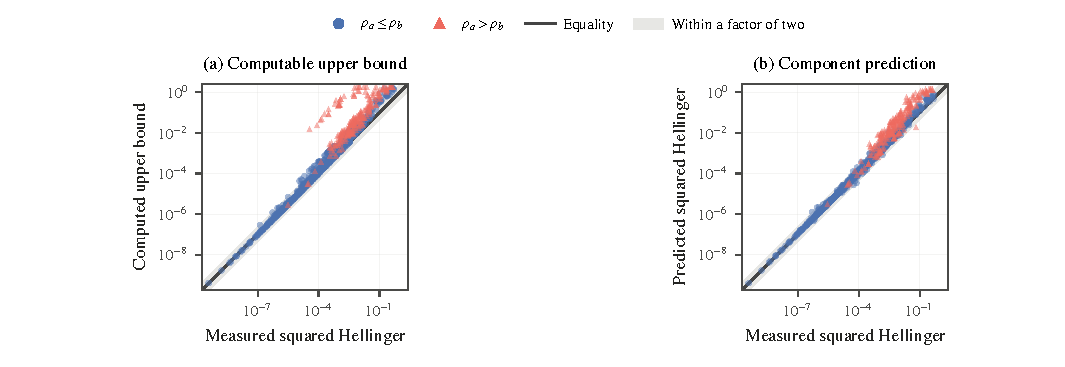
\includegraphics[width=\linewidth]{figures/hierarchy_stability_validation.pdf}
\caption{\textbf{Computable inter-level response diagnostics.}
All 1,080 source-subsampling transitions across six synthetic families and five penalty pairs.
Left: the computable upper bound $B_{\mathrm{comp}}$ against measured error $e$; right: component prediction $\widehat e$ against $e$.
The diagonal denotes equality, and the shaded band spans a factor of two.
Colors and markers distinguish $\rho_a\leq\rho_b$ from $\rho_a>\rho_b$; predictions are less accurate in the latter regime.}
\label{fig:hierarchy-stability-validation}
\end{figure}

\begin{table}[t]
\centering
% CN: 各行由同一 forward_results.json 全量分组重新计算，核对同批 summary.json；精确数值见 figures/hierarchy_stability_validation.json。每组 216 个转换，Overall 为全部 1080 个转换的 pooled 统计，未平均各组中位数。
% EN: Rows are recomputed by grouping the same complete forward_results.json and checked against summary.json in that batch; exact values are in figures/hierarchy_stability_validation.json. Each group has 216 transitions; Overall pools all 1,080 transitions rather than averaging group medians.
\caption{\textbf{Accuracy of inheritance bounds and response predictions.}
Each penalty pair includes 216 transitions from Figure~\ref{fig:hierarchy-stability-validation}.
Bound ratios and prediction fold errors $\max\{\widehat e/e,e/\widehat e\}$ are medians; the final column gives the percentage of predictions within a factor of two.}
\label{tab:stability-diagnostics}
\small
\setlength{\tabcolsep}{7pt}
\begin{tabular}{lrrr}
\toprule
$(\rho_a,\rho_b)$ & $B_{\mathrm{comp}}/e$ & Prediction fold & Within $2\times$ \\
\midrule
$(0.1,0.1)$ & 2.40 & 1.27 & 91.7\% \\
$(1,1)$ & 1.37 & 1.22 & 97.2\% \\
$(10,10)$ & 1.03 & 1.02 & 99.1\% \\
$(0.1,2)$ & 1.05 & 1.00 & 100.0\% \\
$(2,0.1)$ & 6.51 & 3.95 & 20.4\% \\
\midrule
Overall & 1.42 & 1.12 & 81.7\% \\
\bottomrule
\end{tabular}

\end{table}

The computable bound covers the measured error in all 1,080 transitions, with median bound/error ratio $1.42$ and 90th percentile $6.56$.
Its worst ratio is $588$, showing that the bound can remain conservative.
The component predictor has median fold error $1.12$, with $81.7\%$ of predictions within a factor of two and a maximum fold error of $25.26$.
Table~\ref{tab:stability-diagnostics} shows that the $(2,0.1)$ penalty regime accounts for the largest loss of accuracy.
The purely geometric interaction bound is substantially looser, with median bound/error ratio approximately $1{,}281$ on the same transitions.

% CN: 独立证书验证来自同批 full_certificate_results.json，SHA256=d88f688950a3a497ec55b3d6dfc3686caf99b5f6cc3d779d5da7183a77ede789；预测先冻结，再求细层参考；120/120 区间覆盖对应误差，但部分区间较宽。
% EN: Independent certificates come from full_certificate_results.json in the same batch, SHA256=d88f688950a3a497ec55b3d6dfc3686caf99b5f6cc3d779d5da7183a77ede789; predictions are frozen before solving fine references; 120/120 intervals contain the corresponding errors, although some intervals are wide.
A separate 120-transition test freezes predictions before computing the fine references; all returned certificate intervals contain the corresponding reference errors, although some intervals are wide.
These auxiliary computations validate the response diagnostics; they are not production hierarchy steps or measurements of warm-start speedup.

\section{Hyperparameter Sensitivity}
\label{app:uot-parameter-sensitivity}

We vary the hierarchy split factor $s$, dual-assignment budget $\kappa$, pricing budget $\gamma$, and support budget factor $\beta$ one at a time.
The other budget parameters remain at their default values $(s,\kappa,\gamma,\beta)=(4,16,2,10)$, and the coarsest-size threshold is fixed at 256.
The split factor is the reciprocal of the sampling ratio used in \hello, so $s\in\{2,4,8\}$ corresponds to sampling ratios $\{0.5,0.25,0.125\}$.
All settings satisfy $\beta\geq\gamma+3$ and use the same original full-space KKT tolerance of $10^{-6}$.
The common default configuration is measured once per penalty pair and reused across the four blocks, giving 36 distinct runs; all reach the target tolerance.

\begin{table}[t]
\centering
% CN: 全部耗时与显存来自 paper_experiments_uot/parameter_sensitivity/results/20261110_v2_paper_data/summary_table.json；原始指标为同批次 cases/*/*/metrics.json；n=262144，36/36 成功。按 groups.parameter/value 匹配各行；四块共享每组 penalty 的 baseline，显存为 peak_gpu_memory_mib / 1024。
% EN: All runtimes and memory measurements come from paper_experiments_uot/parameter_sensitivity/results/20261110_v2_paper_data/summary_table.json, with raw metrics in cases/*/*/metrics.json; n=262144 and 36/36 runs succeeded. Match rows by groups.parameter/value; blocks share each penalty's baseline, and memory is peak_gpu_memory_mib / 1024.
% \xwz{Safeguard rerun pending: this sensitivity batch used refinement_forcing_check=False and refinement_progress_check=False; replace these measurements after the supported safeguard-enabled rerun.}
\caption{\textbf{Hyperparameter sensitivity across marginal penalties.}
TOME E11.5$\to$E12.5 with $m=n=262{,}144$, $d=30$, seed 42, and one measurement per configuration at KKT tolerance $10^{-6}$.
\runtime is in seconds; \gpumem is peak active GPU allocation in GiB.
Each block varies one parameter; bold and underlined entries mark the best and second-best displayed values within that block and penalty setting.}
\label{tab:uot-parameter-sensitivity}
\small
\setlength{\tabcolsep}{3pt}
\begin{tabular}{@{}l cc cc cc cc@{}}
\toprule
\multirow{2}{*}{Variant} & \multicolumn{2}{c}{$(0.1,0.1)$} & \multicolumn{2}{c}{$(1,1)$} & \multicolumn{2}{c}{$(10,10)$} & \multicolumn{2}{c}{$(0.045,99.995)$} \\
\cmidrule(lr){2-3}\cmidrule(lr){4-5}\cmidrule(lr){6-7}\cmidrule(lr){8-9}
 & \runtime & \gpumem & \runtime & \gpumem & \runtime & \gpumem & \runtime & \gpumem \\
\midrule
\multicolumn{9}{l}{\textit{(a) Hierarchy split factor $s$ ($\kappa=16,\gamma=2,\beta=10$)}} \\
$s=2$ & 16.54 & \textbf{1.631} & 18.49 & \textbf{1.600} & \underline{26.61} & \textbf{1.591} & 16.29 & \textbf{1.637} \\
$s=4$ & \underline{12.76} & \underline{1.659} & \underline{14.18} & \underline{1.630} & \textbf{20.15} & 1.621 & \underline{11.65} & \underline{1.658} \\
$s=8$ & \textbf{10.55} & 1.697 & \textbf{13.11} & 1.664 & 26.92 & \underline{1.611} & \textbf{10.36} & 1.696 \\
\midrule
\multicolumn{9}{l}{\textit{(b) Dual-assignment budget $\kappa$ ($s=4,\gamma=2,\beta=10$)}} \\
$\kappa=8$ & \underline{14.05} & \textbf{0.995} & \underline{15.99} & \textbf{0.981} & \underline{22.25} & \textbf{0.979} & \underline{14.13} & \textbf{0.998} \\
$\kappa=16$ & \textbf{12.76} & \underline{1.659} & \textbf{14.18} & \underline{1.630} & \textbf{20.15} & \underline{1.621} & \textbf{11.65} & \underline{1.658} \\
$\kappa=32$ & 14.59 & 3.063 & 20.83 & 3.008 & 39.61 & 2.997 & 14.65 & 3.071 \\
\midrule
\multicolumn{9}{l}{\textit{(c) Pricing budget $\gamma$ ($s=4,\kappa=16,\beta=10$)}} \\
$\gamma=1$ & \textbf{11.84} & \textbf{1.659} & \textbf{13.19} & \textbf{1.630} & \textbf{18.96} & \textbf{1.620} & \textbf{10.59} & \textbf{1.658} \\
$\gamma=2$ & \underline{12.76} & \textbf{1.659} & \underline{14.18} & \textbf{1.630} & \underline{20.15} & \underline{1.621} & \underline{11.65} & \textbf{1.658} \\
$\gamma=4$ & 14.18 & \textbf{1.659} & 15.05 & \textbf{1.630} & 21.26 & \underline{1.621} & 12.66 & \textbf{1.658} \\
\midrule
\multicolumn{9}{l}{\textit{(d) Support budget factor $\beta$ ($s=4,\kappa=16,\gamma=2$)}} \\
$\beta=5$ & \underline{12.67} & \textbf{1.657} & \textbf{13.96} & \textbf{1.628} & \textbf{19.83} & \underline{1.623} & \textbf{11.48} & 1.661 \\
$\beta=10$ & 12.76 & \underline{1.659} & 14.18 & \underline{1.630} & \underline{20.15} & \textbf{1.621} & \underline{11.65} & \textbf{1.658} \\
$\beta=20$ & \textbf{12.05} & 1.660 & \underline{14.03} & \textbf{1.628} & 20.21 & \textbf{1.621} & 11.66 & \underline{1.659} \\
\bottomrule
\end{tabular}
\end{table}

% \xwz{Temporarily omit the historical runtime-breakdown section; rerun and audit non-overlapping timers before restoring.}
% \section{Runtime Breakdown}
% \label{app:runtime-breakdown}
%
% We separate end-to-end runtime into hierarchy construction and initialization, restricted solves, full scans, support updates, and remaining overhead.
% The first category includes hierarchy preparation, dual propagation, potential translation, and initial support construction across all levels.
% Restricted time counts the inner solver only; support-update time includes insertion, deduplication, budgeted pruning, and triggered sparsification, with each operation counted once.
% Full-scan time counts each complete-edge traversal once, including fused candidate selection and violation evaluation.
% The remaining overhead is the end-to-end time not assigned to these categories, making their sum equal the reported total.
% This partition requires non-overlapping timing scopes; nested sparsification or initialization timers must be separated before aggregation.
% Compilation warm-up and common post-solve evaluation are excluded as in the main comparison.
%
% \begin{table}[t]
% \centering
% % CN: n=16384 来自 paper_experiments_uot/accuracy_runtime_pareto/results/20261025_222731/cases/n16384_rhoa*_rhob*_seed42/shuttle_tolerance_1e-06_repeat0/metrics.json；n=65536 来自 paper_experiments_uot/component_ablation/results/20261102_193809/cases/n65536_rhoa*_rhob*_seed42/shuttle_fixed_repeat0/metrics.json。
% % EN: n=16384 uses paper_experiments_uot/accuracy_runtime_pareto/results/20261025_222731/cases/n16384_rhoa*_rhob*_seed42/shuttle_tolerance_1e-06_repeat0/metrics.json; n=65536 uses paper_experiments_uot/component_ablation/results/20261102_193809/cases/n65536_rhoa*_rhob*_seed42/shuttle_fixed_repeat0/metrics.json.
% % CN: Init=hierarchy_build_time+各层 initialization_time；Restricted=粗层 diagnostics.restricted_time+各细层 iteration.restricted_time；Scan/Update 累加对应迭代计时；Other 为 runtime_sec 减去前四项。未记录触发的 sparsification；舍入后的 Other 吸收最多毫秒级的舍入差。
% % EN: Init sums hierarchy_build_time and level initialization_time; Restricted sums coarsest diagnostics.restricted_time and refined iteration.restricted_time; Scan/Update sum their iteration timers; Other is the runtime_sec remainder. No triggered sparsification was recorded; rounded Other absorbs millisecond-scale rounding differences.
% % \xwz{RERUN REQUIRED: these are approximate layout values extracted from historical runs with different source versions. Rerun the current production solver on a common unshared-GPU protocol and audit non-overlapping timer scopes before treating this table as a final runtime breakdown.}
% \caption{\textbf{End-to-end runtime breakdown for \ours.}
% Preliminary historical timings on TOME E11.5$\to$E12.5 with $d=30$ and $m=n$.
% Init includes hierarchy construction and initialization; Update includes triggered sparsification.
% All component entries are seconds, and their sum equals Total.}
% \label{tab:uot-runtime-breakdown}
% \small
% \setlength{\tabcolsep}{5pt}
% \begin{tabular}{rlrrrrrr}
% \toprule
% $n$ & $(\rho_a,\rho_b)$ & Init & Restricted & Scan & Update & Other & Total \\
% \midrule
% \multirow{4}{*}{$2^{14}$} & $(0.1,0.1)$ & 0.131 & 1.581 & 0.062 & 0.015 & 0.057 & 1.846 \\
%  & $(1,1)$ & 0.124 & 2.287 & 0.068 & 0.018 & 0.034 & 2.531 \\
%  & $(10,10)$ & 0.123 & 7.139 & 0.133 & 0.050 & 0.050 & 7.495 \\
%  & $(0.045,99.995)$ & 0.113 & 1.626 & 0.057 & 0.011 & 0.030 & 1.837 \\
% \midrule
% \multirow{4}{*}{$2^{16}$} & $(0.1,0.1)$ & 0.552 & 2.666 & 0.575 & 0.022 & 0.044 & 3.859 \\
%  & $(1,1)$ & 0.592 & 5.854 & 0.592 & 0.028 & 0.053 & 7.119 \\
%  & $(10,10)$ & 0.584 & 23.108 & 0.914 & 0.066 & 0.089 & 24.761 \\
%  & $(0.045,99.995)$ & 0.600 & 2.901 & 0.595 & 0.021 & 0.044 & 4.161 \\
% \bottomrule
% \end{tabular}
%
% \smallskip
% % \xwz{Placeholder: finalize the profiled sizes and seed counts, and insert exact source paths.
% % If additional timing instrumentation is needed to separate nested scopes, add it before reporting this partition; do not interpret missing timers as zero cost.}
% \end{table}

\section{UFGW Solver Trajectories}
\label{app:ufgw-solver-trajectories}

We record the common objective at initialization and after each of ten complete coupling-update sweeps for the STARmap comparison in Table~\ref{tab:ufgw-solvers}.
Figure~\ref{fig:ufgw-objective-time} uses the same independent FP64 objective for both methods and excludes its evaluation from the plotted runtime.
Each panel shows the original objective on a linear scale, with an inset enlarging sweeps 3--10 using shared axis limits for both methods.
The zero-entropy comparison reaches a lower final objective with \oursufgw, while the entropic comparison reaches nearly identical final objectives.
These trajectories describe progress under the fixed sweep budget rather than certify outer convergence or global optimality.

\begin{figure*}[t]
\centering
% CN: 左图来自 /home/xiawenzhou/project/hierarchical_ot/paper_experiments_uot/ufgw_solver_comparison/results/20261110_ufgw_starmap_n16384/objective_time_n16384_eps0_rhoa0.1_rhob0.1_alpha0.4.pdf；原始曲线为同批 cases/n16384_rhoa0.1_rhob0.1_eps0_seed0/{shuttle,pot}_repeat0/trajectory.json。
% EN: Left panel: /home/xiawenzhou/project/hierarchical_ot/paper_experiments_uot/ufgw_solver_comparison/results/20261110_ufgw_starmap_n16384/objective_time_n16384_eps0_rhoa0.1_rhob0.1_alpha0.4.pdf; raw curves: cases/n16384_rhoa0.1_rhob0.1_eps0_seed0/{shuttle,pot}_repeat0/trajectory.json in the same batch.
% CN: 原始 objective 与 inset 纵轴范围见同批 trajectory_plot_data.json；主图与 inset 均不平移或归一化数值。
% EN: Raw objectives and inset vertical limits are recorded in trajectory_plot_data.json in the same batch; neither view shifts or normalizes values.
\begin{subfigure}[t]{0.49\textwidth}
\centering
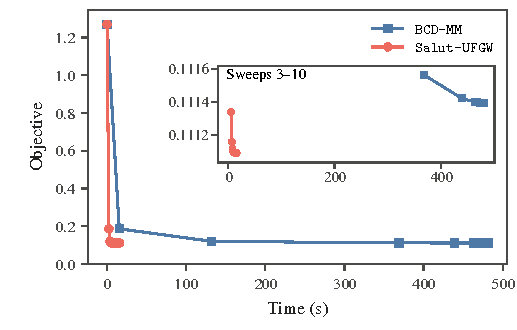
\includegraphics[width=\linewidth]{figures/ufgw_objective_time_eps0.pdf}
\caption{$\varepsilon=0$.}
\end{subfigure}\hfill
% CN: 右图来自同批 objective_time_n16384_eps0.001_rhoa0.1_rhob0.1_alpha0.4.pdf；原始曲线为 cases/n16384_rhoa0.1_rhob0.1_eps0.001_seed0/{shuttle,pot}_repeat0/trajectory.json；图由 collect.py --batch-id 20261110_ufgw_starmap_n16384 生成。
% EN: Right panel: objective_time_n16384_eps0.001_rhoa0.1_rhob0.1_alpha0.4.pdf in the same batch; raw curves: cases/n16384_rhoa0.1_rhob0.1_eps0.001_seed0/{shuttle,pot}_repeat0/trajectory.json; generated by collect.py --batch-id 20261110_ufgw_starmap_n16384.
\begin{subfigure}[t]{0.49\textwidth}
\centering
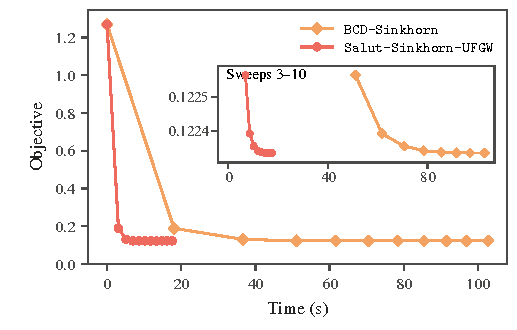
\includegraphics[width=\linewidth]{figures/ufgw_objective_time_eps0.001.pdf}
\caption{$\varepsilon=10^{-3}$.}
\end{subfigure}
\caption{\textbf{UFGW objective--time trajectories.}
STARmap well05--well11 with $m=n=16{,}384$, $\alpha=0.4$, and $\rho_a=\rho_b=0.1$.
Markers show initialization and ten complete sweeps; the initial product couplings are assigned time zero.
Left: \oursufgw versus \bcdmm; right: \ourssinkhornufgw versus \bcdsinkhorn.
Main plots show the original objective on linear axes; insets enlarge sweeps 3--10 with shared axis limits for both methods.
Results use seed $0$ with one measurement per configuration on A100 GPUs.}
\label{fig:ufgw-objective-time}
\end{figure*}

% \xwz{Temporarily omit the unmeasured Schmitzer/LCN baseline section; restore only with measured results.}
% \section{Additional Entropic UOT Baselines}
% \label{app:entropic-additional-baselines}
%
% We extend the main entropic comparison with Schmitzer's multiscale KL solver and LCN clustering followed by generalized sparse \sinkhorn.
% Schmitzer uses the official CPU implementation with stabilization, kernel truncation, and entropy scaling; its CPU memory is reported separately from GPU memory.
% The LCN baseline uses the adapted clustering-only support construction and sparse UOT updates, without the global low-rank component of the full LCN method.
% All methods are evaluated against the same entropic objective and full-space gap~\eqref{eq:entropic-evaluation-gap}.
% Support construction, hierarchy construction, sampling, and sparse iterations are included in total solver runtime, with preprocessing conventions and arithmetic precision disclosed for each implementation.
%
% \begin{table}[t]
% \centering
% % CN: 占位；待填 paper_experiments/entropic_uot/results/<batch>/summary.csv，包含 Schmitzer 与 LCN 适配版本。
% % EN: Placeholder; insert paper_experiments/entropic_uot/results/<batch>/summary.csv, including the Schmitzer and adapted LCN baselines.
% \caption{\textbf{Additional entropic UOT baseline comparison.}
% % \xwz{PLACEHOLDER: fix a shared $(n,d,\rho_a,\rho_b,\varepsilon)$ and specify memory measurement scopes before reporting results.}
% CPU and GPU memory use separate columns; an inapplicable measurement is marked n/a rather than zero.}
% \label{tab:entropic-additional-baselines}
% \small
% \setlength{\tabcolsep}{7pt}
% \begin{tabular}{lrrrr}
% \toprule
% Method & \runtime~$\downarrow$ & GPU memory & CPU memory & \entropicgap~$\downarrow$ \\
% \midrule
% \ourssparsink & -- & -- & -- & -- \\
% OTT-online & -- & -- & -- & -- \\
% Spar-Sink & -- & -- & -- & -- \\
% Schmitzer (CPU) & -- & n/a & -- & -- \\
% LCN clustering + sparse \sinkhorn & -- & -- & -- & -- \\
% \bottomrule
% \end{tabular}
% \end{table}
%
% \paragraph{Extended numerical results.}
% % \xwz{Add the complete entropic runtime--accuracy and memory-scaling plots here, including Schmitzer and LCN, with separate panels for each fixed entropic objective.
% % Add larger-scale UFGW runs that exceed the common baseline size range if needed.
% % Record exact data paths in each table or figure source comment when replacing placeholders.}
